% patch_gp_slides.tex
% Patch GP: GP-based Lossy Compression of Scientific Datasets
% Audience: lossy compression researcher (mentor/collaborator) + postdoc
\documentclass[10pt]{beamer}
\usetheme{Madrid}
\usecolortheme{seahorse}
\usepackage{amsmath,amssymb,bm}
\usepackage{tikz}
\usetikzlibrary{patterns,arrows.meta,decorations.pathreplacing,calc}
\usepackage{booktabs}
\usepackage{graphicx}
\usepackage{xcolor}

% colour palette
\definecolor{myblue}{RGB}{31,119,180}
\definecolor{myorange}{RGB}{255,127,14}
\definecolor{mygreen}{RGB}{44,160,44}
\definecolor{mygray}{RGB}{127,127,127}

\setbeamertemplate{navigation symbols}{}
\setbeamertemplate{footline}[frame number]

% ─── title ────────────────────────────────────────────────────────────────────
\title[Patch GP Compression]{%
  Patch GP: Gaussian Process–Based Lossy Compression\\
  of Scientific Datasets}
\subtitle{Hurricane ISABEL W Field Case Study}
\author{Jessie Chen}
\institute{NC State University / Argonne National Laboratory}
\date{\today}

\begin{document}

\begin{frame}
  \titlepage
\end{frame}

% ─── outline ──────────────────────────────────────────────────────────────────
\begin{frame}{Outline}
  \tableofcontents
\end{frame}

% ══════════════════════════════════════════════════════════════════════════════
\section{Motivation}
% ══════════════════════════════════════════════════════════════════════════════
\begin{frame}{Motivation}
  \begin{itemize}
    \item Scientific simulations produce \textbf{large floating-point arrays}
          (e.g.\ Hurricane ISABEL: $100\times500\times500\approx25$M values).
    \item Lossy compression under an \textbf{absolute error bound} (EB) is
          the standard regime: every reconstructed value satisfies
          $|\hat{f}(\mathbf{x})-f(\mathbf{x})|\leq\mathrm{EB}$.
    \item State-of-the-art: \textbf{SZ3 ALGO\_INTERP} — hierarchical dyadic
          cubic-spline prediction followed by quantisation and entropy coding.
          Fast and effective, but uses a \emph{fixed predictor}.
    \item \textbf{Our goal:} replace the fixed interpolant with a
          \emph{Gaussian Process} (GP) that
          \begin{enumerate}
            \item adapts its predictor to the data's spatial covariance;
            \item selects anchor points (raw-stored values)
                  \emph{optimally} via randomised pivoted Cholesky (RPCholesky);
            \item propagates quantisation uncertainty through the noise model.
          \end{enumerate}
  \end{itemize}
\end{frame}

% ══════════════════════════════════════════════════════════════════════════════
\section{Background: SZ3 ALGO\_INTERP}
% ══════════════════════════════════════════════════════════════════════════════
\begin{frame}{SZ3 ALGO\_INTERP --- Baseline}
  \begin{columns}
    \column{0.55\textwidth}
    \begin{enumerate}
      \item Place coarse anchor grid at stride $s$ (power of 2).
            Store all anchors as \textbf{raw float32}.
      \item At each level $k$: predict midpoints along $X\!\to\!Y\!\to\!Z$
            by cubic-spline interpolation from 4 nearest known values.
      \item Quantise residual:
            $q = \lfloor e\,/\,(2\cdot\mathrm{EB})\rceil$,\;
            store $q$ (entropy coded).
      \item Use \emph{reconstructed} value $\hat{f}+q\cdot2\cdot\mathrm{EB}$
            as input for subsequent predictions.
      \item Repeat until all $N$ values resolved.
    \end{enumerate}
    \vspace{4pt}
    \textbf{Key property:} total work $O(N)$; predictor has no
    free parameters; \emph{no} anchor selection.
    \column{0.42\textwidth}
    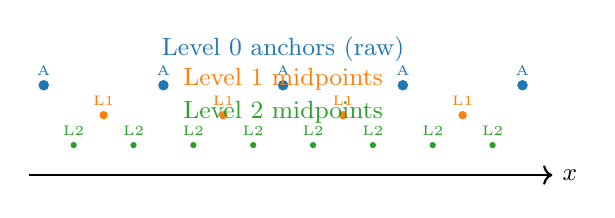
\begin{tikzpicture}[scale=0.38]
      % 1D schematic of dyadic levels
      \foreach \x in {0,4,8,12,16}
        \fill[myblue] (\x,3) circle (5pt) node[above,font=\tiny]{A};
      \foreach \x in {2,6,10,14}
        \fill[myorange] (\x,2) circle (4pt) node[above,font=\tiny]{L1};
      \foreach \x in {1,3,5,7,9,11,13,15}
        \fill[mygreen] (\x,1) circle (3pt) node[above,font=\tiny]{L2};
      \draw[thick,->] (-0.5,0)--(17,0) node[right,font=\small]{$x$};
      \node[font=\small,myblue] at (8,4.2) {Level 0 anchors (raw)};
      \node[font=\small,myorange] at (8,3.2) {Level 1 midpoints};
      \node[font=\small,mygreen] at (8,2.1) {Level 2 midpoints};
    \end{tikzpicture}
  \end{columns}
\end{frame}

% ══════════════════════════════════════════════════════════════════════════════
\section{Patch GP Algorithm}
% ══════════════════════════════════════════════════════════════════════════════
\begin{frame}{Patch GP --- Overview}
  \begin{block}{Core idea}
    Tile the volume into a two-level spatial partition.
    The \emph{center} of each inner block is an \textbf{anchor candidate}.
    A GP with RPCholesky sensor selection then processes blocks
    in $K$ rounds, one inner-block position per round.
  \end{block}
  \vspace{4pt}
  \begin{columns}
    \column{0.48\textwidth}
    \textbf{What stays the same as SZ3:}
    \begin{itemize}
      \item Absolute error bound EB
      \item Quantisation: $q=\lfloor e/(2\cdot\mathrm{EB})\rceil$
      \item Reconstructed values feed subsequent predictions
      \item Entropy coding of all $q$-bins
    \end{itemize}
    \column{0.48\textwidth}
    \textbf{What changes:}
    \begin{itemize}
      \item Predictor: GP (Matérn-5/2, tuned HPs)
      \item Anchor selection: RPCholesky+GKS (space-filling)
      \item Noise model: $\sigma_n=\mathrm{EB}/\sigma_y$ for pseudo-anchors
      \item Processing order: patch-by-patch, not dyadic level
    \end{itemize}
  \end{columns}
\end{frame}

% ─── patch structure diagram ───────────────────────────────────────────────────
\begin{frame}{Patch Structure (2-D Illustration)}
  \centering
  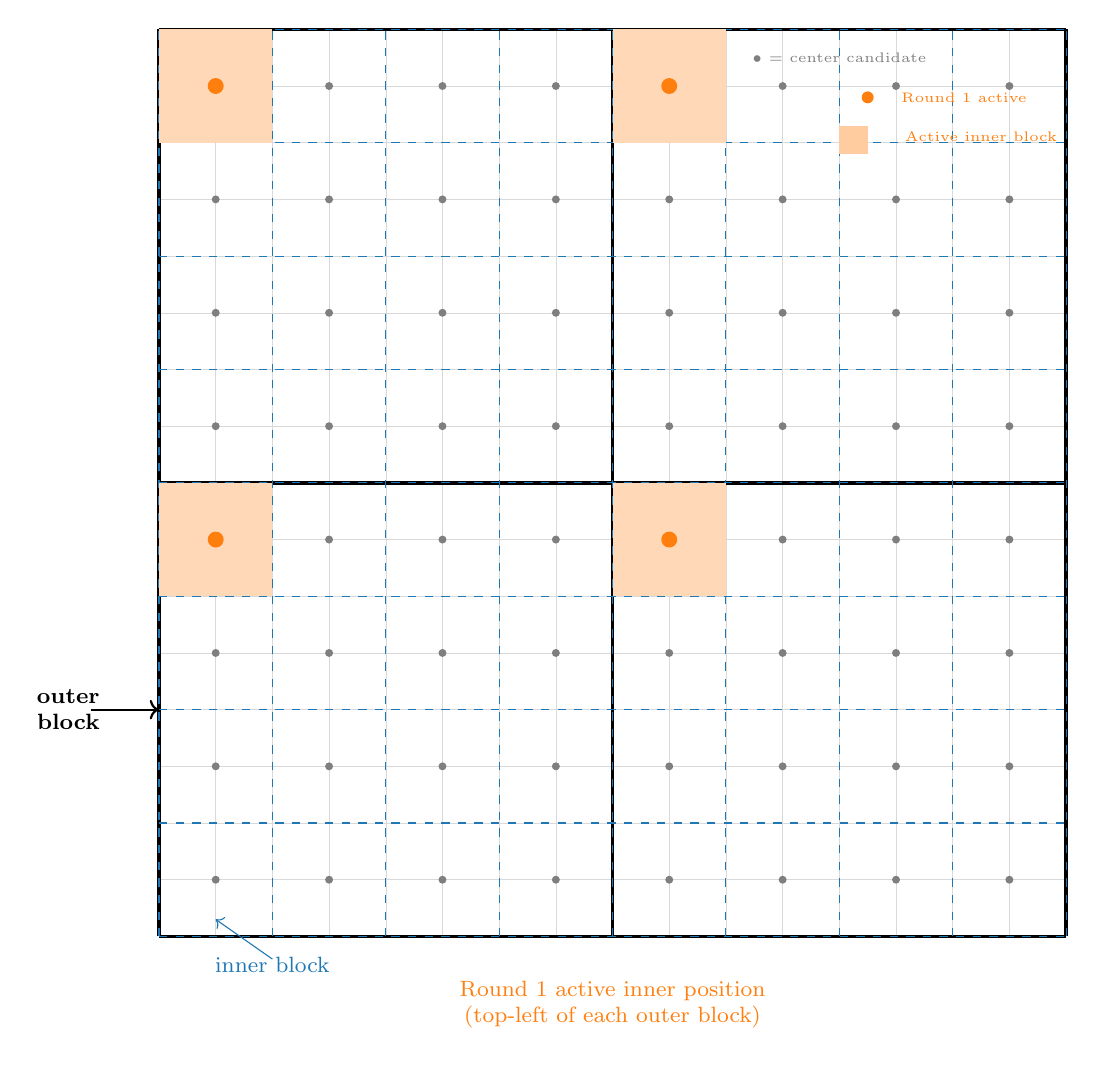
\begin{tikzpicture}[scale=0.72]
    % --- outer grid 4x4 outer blocks, each 4x4 inner blocks of 1x1 ---
    % Draw 16x16 fine grid
    \foreach \x in {0,...,16}
      \draw[gray!30,very thin] (\x,0)--(\x,16);
    \foreach \y in {0,...,16}
      \draw[gray!30,very thin] (0,\y)--(16,\y);

    % Outer block boundaries (4 outer blocks in 4x4 arrangement)
    \foreach \x in {0,8,16}
      \draw[black,very thick] (\x,0)--(\x,16);
    \foreach \y in {0,8,16}
      \draw[black,very thick] (0,\y)--(16,\y);

    % Inner block boundaries (4x4 inner per outer)
    \foreach \x in {0,2,4,6,8,10,12,14,16}
      \draw[myblue,thin,dashed] (\x,0)--(\x,16);
    \foreach \y in {0,2,4,6,8,10,12,14,16}
      \draw[myblue,thin,dashed] (0,\y)--(16,\y);

    % Highlight Round 1 inner position (top-left inner of every outer block)
    \foreach \ox in {0,8} {
      \foreach \oy in {0,8} {
        \fill[myorange!30] (\ox,\oy+6) rectangle (\ox+2,\oy+8);
      }
    }

    % Center points of all inner blocks (dots)
    \foreach \ox in {0,8} {
      \foreach \oy in {0,8} {
        \foreach \ix in {0,2,4,6} {
          \foreach \iy in {0,2,4,6} {
            \fill[mygray] (\ox+\ix+1, \oy+\iy+1) circle (2pt);
          }
        }
      }
    }

    % Highlight Round 1 centers (anchors / predicted)
    \foreach \ox in {0,8} {
      \foreach \oy in {0,8} {
        \fill[myorange] (\ox+1, \oy+7) circle (4pt);
      }
    }

    % Labels
    \node[font=\footnotesize,myblue] at (2,-0.5) {inner block};
    \draw[myblue,->] (2,-0.4)--(1.0,0.3);

    \node[font=\footnotesize,black,align=center] at (-1.6,4)
      {\textbf{outer}\\\textbf{block}};
    \draw[thick,->] (-1.2,4)--(0,4);

    \node[font=\footnotesize,myorange,align=center] at (8,-1.2)
      {Round 1 active inner position\\(top-left of each outer block)};

    \node[font=\tiny,mygray] at (12,15.5) {$\bullet$ = center candidate};
    \fill[myorange] (12.5,14.8) circle (3pt);
    \node[font=\tiny,myorange] at (14.2,14.8) {Round 1 active};

    \fill[myorange!40] (12,13.8) rectangle (12+0.5,13.8+0.5);
    \node[font=\tiny,myorange] at (14.5,14.1) {Active inner block};
  \end{tikzpicture}

  \vspace{4pt}
  {\small
    Each outer block contains $4\times4$ inner blocks (here shown in 2-D).\\
    In 3-D: outer $= P_{\!xy}\!\times\!P_{\!xy}\!\times\!P_z$;
    inner $= (P_{\!xy}/4)\!\times\!(P_{\!xy}/4)\!\times\!(P_z/4)$.\;
    $P_{\!xy}$ chosen $\le \ell_{xy}\cdot N_y$;
    $P_z$ chosen $\le \ell_z\cdot N_z$.}
\end{frame}

% ─── round-by-round ────────────────────────────────────────────────────────────
\begin{frame}{Round-by-Round Processing}
  \centering
  % Draw 4 rounds side-by-side using explicit coordinates (no nested \def/\foreach)
  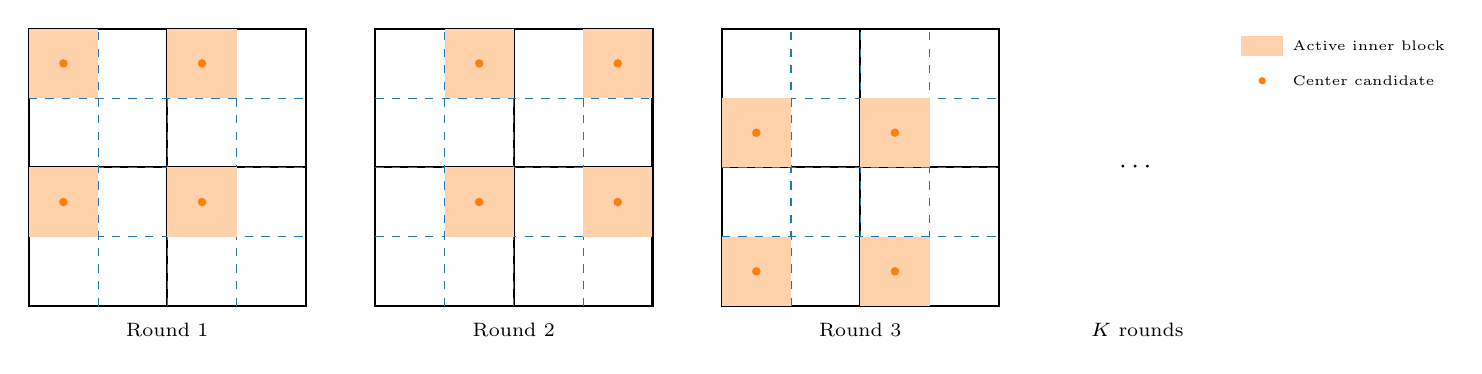
\begin{tikzpicture}[scale=0.44]
    % Helper: each "panel" is 8x8 units; panels are at xoff = 0, 10, 20, 30

    % ---- PANEL 1: Round 1 (active inner pos top-left of each outer) ----
    % outer+inner grid
    \draw[black,thick] (0,0) rectangle (8,8);
    \draw[black,thick] (4,0)--(4,8); \draw[black,thick] (0,4)--(8,4);
    \foreach \d in {2,4,6}{ \draw[myblue,dashed,thin] (\d,0)--(\d,8); \draw[myblue,dashed,thin] (0,\d)--(8,\d); }
    % active inner: top-left of each outer (inner pos (0,1) = y=6..8)
    \fill[myorange!35] (0,6) rectangle (2,8); \fill[myorange!35] (4,6) rectangle (6,8);
    \fill[myorange!35] (0,2) rectangle (2,4); \fill[myorange!35] (4,2) rectangle (6,4);
    % centers
    \fill[myorange] (1,7) circle (3.5pt); \fill[myorange] (5,7) circle (3.5pt);
    \fill[myorange] (1,3) circle (3.5pt); \fill[myorange] (5,3) circle (3.5pt);
    \node[font=\scriptsize,align=center] at (4,-0.7) {Round 1};

    % ---- PANEL 2: Round 2 (active inner pos second column) ----
    \draw[black,thick] (10,0) rectangle (18,8);
    \draw[black,thick] (14,0)--(14,8); \draw[black,thick] (10,4)--(18,4);
    \foreach \d in {2,4,6}{ \draw[myblue,dashed,thin] (10+\d,0)--(10+\d,8); \draw[myblue,dashed,thin] (10,\d)--(18,\d); }
    \fill[myorange!35] (12,6) rectangle (14,8); \fill[myorange!35] (16,6) rectangle (18,8);
    \fill[myorange!35] (12,2) rectangle (14,4); \fill[myorange!35] (16,2) rectangle (18,4);
    \fill[myorange] (13,7) circle (3.5pt); \fill[myorange] (17,7) circle (3.5pt);
    \fill[myorange] (13,3) circle (3.5pt); \fill[myorange] (17,3) circle (3.5pt);
    \node[font=\scriptsize,align=center] at (14,-0.7) {Round 2};

    % ---- PANEL 3: Round 3 (active inner pos second row) ----
    \draw[black,thick] (20,0) rectangle (28,8);
    \draw[black,thick] (24,0)--(24,8); \draw[black,thick] (20,4)--(28,4);
    \foreach \d in {2,4,6}{ \draw[myblue,dashed,thin] (20+\d,0)--(20+\d,8); \draw[myblue,dashed,thin] (20,\d)--(28,\d); }
    \fill[myorange!35] (20,4) rectangle (22,6); \fill[myorange!35] (24,4) rectangle (26,6);
    \fill[myorange!35] (20,0) rectangle (22,2); \fill[myorange!35] (24,0) rectangle (26,2);
    \fill[myorange] (21,5) circle (3.5pt); \fill[myorange] (25,5) circle (3.5pt);
    \fill[myorange] (21,1) circle (3.5pt); \fill[myorange] (25,1) circle (3.5pt);
    \node[font=\scriptsize,align=center] at (24,-0.7) {Round 3};

    % ---- ellipsis ----
    \node[font=\normalsize] at (32,4) {$\cdots$};
    \node[font=\scriptsize] at (32,-0.7) {$K$ rounds};

    % legend
    \fill[myorange!35] (35,7.2) rectangle (36.2,7.8);
    \node[font=\tiny,right] at (36.2,7.5) {Active inner block};
    \fill[myorange] (35.6,6.5) circle (3pt);
    \node[font=\tiny,right] at (36.2,6.5) {Center candidate};
  \end{tikzpicture}

  \vspace{4pt}
  \begin{itemize}
    \item In each round: \textbf{same inner-block position} from \emph{every} outer block.
    \item RPCholesky sees $M$ center candidates \emph{spread across the volume}
          $\Rightarrow$ good global space-filling selection.
    \item After $K$ rounds: \textbf{all $N$ values resolved}.
  \end{itemize}
\end{frame}

% ─── algorithm box ─────────────────────────────────────────────────────────────
\begin{frame}{Patch GP Algorithm}
  \begin{block}{Notation}
    $M$ outer blocks;\; $K$ rounds;\;
    $\mathcal{C}_r$ = center candidates in round $r$;\;
    $\mathcal{B}_{r,m}$ = non-center pixels of outer block $m$ in round $r$.
  \end{block}
  \vspace{2pt}
  \begin{enumerate}
    \item Fit HP $(\ell_{xy},\ell_z,\sigma^2)$ on $\sim\!600$ random samples (L-BFGS-B MLE)
    \item Compute patch sizes from $\ell_{xy},\ell_z$ (largest divisors $\le$ one length scale)
    \item \textbf{For} $r = 1,\ldots,K$:
    \begin{itemize}
      \item[\textbf{A.}] \textbf{Centers:} RPCholesky selects $\lfloor\alpha M\rceil$ anchors from $\mathcal{C}_r$; store raw float32.
            GP predicts remaining centers; quantise $q_i=\lfloor e_i/(2\,\mathrm{EB})\rceil$.
            Add reconstructed values to conditioning set.
      \item[\textbf{B.}] \textbf{Interiors:} GP predicts all $\bigcup_m \mathcal{B}_{r,m}$ (K\_LOCAL nearest nbrs).
            Quantise; add reconstructed values to conditioning set.
    \end{itemize}
    \item Compute entropy $H$ of all $q$-bins;\; bit rate $= (32\,N_\mathrm{anc} + H\,N_\mathrm{pred})/N$
  \end{enumerate}
\end{frame}

% ─── noise model ───────────────────────────────────────────────────────────────
\begin{frame}{Heteroscedastic Noise Model}
  \begin{columns}
    \column{0.5\textwidth}
    \textbf{GP posterior mean}
    \[
      \mu(\mathbf{x}^*) = \mathbf{k}^*{}^\top
        \bigl(\mathbf{K}+\bm{\Sigma}_n\bigr)^{-1}\mathbf{y}
    \]
    where $\bm{\Sigma}_n = \mathrm{diag}(\sigma_{n,i}^2)$ is
    \emph{per-point} noise.
    \vspace{8pt}

    \begin{tabular}{ll}
      \toprule
      Point type & $\sigma_{n,i}$ \\
      \midrule
      True anchor (float32) & $\approx 0$ \\
      Pseudo-anchor (quantised) & $\mathrm{EB}/\hat{\sigma}_y$ \\
      \bottomrule
    \end{tabular}

    \column{0.47\textwidth}
    \textbf{Why this matters:}
    \begin{itemize}
      \item Quantised values are known only to $\pm\mathrm{EB}$.
      \item Propagating that uncertainty into the posterior
            gives honest confidence intervals.
      \item SZ3 cannot do this — it has no noise model.
      \item Larger EB $\Rightarrow$ larger $\sigma_n$
            $\Rightarrow$ GP naturally deweights noisy pseudo-anchors.
    \end{itemize}
  \end{columns}
\end{frame}

% ─── key differences ───────────────────────────────────────────────────────────
\begin{frame}{Patch GP vs SZ3 ALGO\_INTERP: Key Differences}
  \centering
  \small
  \begin{tabular}{lll}
    \toprule
    & \textbf{SZ3 ALGO\_INTERP} & \textbf{Patch GP} \\
    \midrule
    Predictor & Cubic spline (4 pts) & GP, Matérn-5/2 (K\_LOCAL pts) \\
    Anchor placement & Fixed coarse grid & RPCholesky (space-filling) \\
    Anchor fraction & 100\% of coarse grid & $\alpha=10\%$ of candidates \\
    Noise model & None & Heteroscedastic ($\sigma_n=\mathrm{EB}/\sigma_y$) \\
    HP tuning & None & Global MLE ($\sim$600 pts) \\
    Processing order & Dyadic levels (X$\to$Y$\to$Z) & Patch rounds \\
    Computational cost & $O(N)$ & $O(N\cdot K_\mathrm{local}^3)$ \\
    \bottomrule
  \end{tabular}
\end{frame}

% ══════════════════════════════════════════════════════════════════════════════
\section{Experiment Setup}
% ══════════════════════════════════════════════════════════════════════════════
\begin{frame}{Experiment Setup}
  \begin{columns}
    \column{0.5\textwidth}
    \textbf{Dataset}
    \begin{itemize}
      \item Hurricane ISABEL simulation (NCAR)
      \item Field: vertical wind velocity W
      \item Dimensions: $100\times500\times500$
            ($N=25{,}000{,}000$ values)
      \item Format: float32 ($\approx95$ MB raw)
    \end{itemize}
    \vspace{6pt}
    \textbf{Error bounds tested}
    \[
      \mathrm{EB}\in\{0.005,\,0.01,\,0.02,\,0.05,\,0.1\}
    \]
    \column{0.47\textwidth}
    \textbf{Patch GP settings}
    \begin{itemize}
      \item Kernel: anisotropic Matérn-5/2
      \item HP fitting: 600 pts, L-BFGS-B
      \item Anchor fraction $\alpha=0.10$
      \item $K_\mathrm{local}=20$ nearest neighbours
      \item Patch sizes: data-adaptive
            (largest divisor of 500/100 $\le\ell\cdot N_\mathrm{dim}$)
      \item Outer mult = 4
    \end{itemize}
    \vspace{6pt}
    \textbf{Baseline}
    \begin{itemize}
      \item SZ3 v3 ALGO\_INTERP (cubic spline)
    \end{itemize}
  \end{columns}
  \vspace{6pt}
  \textbf{Metrics:} PSNR (dB), bit rate (bpv), compression ratio (CR).
\end{frame}

% ══════════════════════════════════════════════════════════════════════════════
\section{Results}
% ══════════════════════════════════════════════════════════════════════════════
\begin{frame}{Rate–Distortion Curves}
  \begin{center}
    \includegraphics[width=0.82\textwidth]{rd_patch_gp.png}
  \end{center}
  \vspace{-4pt}
  {\small
    Each colored line = Patch GP at one EB; dots = successive rounds.\\
    Black stars = SZ3 ALGO\_INTERP.
    Upper-left is better (higher quality at lower bit rate).}
\end{frame}

\begin{frame}{Quantisation Error Histograms (EB = 0.01)}
  \begin{center}
    \includegraphics[width=0.92\textwidth]{hist_patch_eb0.01.png}
  \end{center}
  \vspace{-4pt}
  {\small Histograms of $q$-bins for GP-predicted points, per round.
    Tight concentration near 0 indicates accurate predictions.
    Step A center predictions (first bar set) are expected to be
    particularly accurate since HPs capture that resolution level.}
\end{frame}

% ══════════════════════════════════════════════════════════════════════════════
\section{Future Work}
% ══════════════════════════════════════════════════════════════════════════════
\begin{frame}{Future Work}
  \begin{enumerate}
    \item \textbf{Local HP fitting per round} — use M center candidates as
          tuning data for round-specific $(\ell_{xy},\ell_z,\sigma^2)$.
    \item \textbf{Adaptive patch sizing} — octree decomposition; finer patches
          in high-variance regions (e.g.\ hurricane eye).
    \item \textbf{Boundary continuity} — Patchwork Kriging
          (Park \& Apley, JMLR 2018) to remove discontinuities at patch edges.
    \item \textbf{Comparison with Progressive GP} — dyadic midpoint version
          (separate script) on same RD axes.
    \item \textbf{SZ3 ALGO\_LORENZO\_REG} as a second baseline.
    \item \textbf{Other fields} — U, V, pressure, temperature from ISABEL.
    \item \textbf{Computational scaling} — batch Cholesky across patches;
          GPU acceleration.
  \end{enumerate}
\end{frame}

% ─── conclusion ────────────────────────────────────────────────────────────────
\begin{frame}{Conclusion}
  \begin{itemize}
    \item Patch GP replaces SZ3's fixed cubic-spline predictor with a
          \textbf{data-adaptive Gaussian Process}.
    \item \textbf{RPCholesky} selects space-filling anchors — reducing raw
          storage relative to SZ3's fixed coarse grid.
    \item \textbf{Heteroscedastic noise} propagates quantisation uncertainty
          honestly through the GP posterior.
    \item The two-level spatial partition enables \textbf{globally-aware
          sensor selection} (M candidates spread across the volume)
          while keeping individual GP solves small.
    \item RD comparison against SZ3 ALGO\_INTERP is in progress.
  \end{itemize}
  \vspace{8pt}
  \begin{block}{Key references}
    \small
    Park \& Apley (2018). \textit{Patchwork Kriging for Large-scale GP Regression.} JMLR.\\
    Datta et al.\ (2016). \textit{Hierarchical Nearest-Neighbour GP Models.} JASA.\\
    SZ3: Liang et al.\ (2022). \textit{SZ3: A modular framework for composing prediction-based error-bounded lossy compressors.} IEEE TPDS.
  \end{block}
\end{frame}

\end{document}
